\documentclass[letterpaper]{article} % DO NOT CHANGE THIS
\usepackage[submission]{aaai2027} % DO NOT CHANGE THIS
\usepackage[hyphens]{url} % DO NOT CHANGE THIS
\usepackage{graphicx} % DO NOT CHANGE THIS
\urlstyle{rm} % DO NOT CHANGE THIS
\def\UrlFont{\rm} % DO NOT CHANGE THIS
\usepackage{natbib} % DO NOT CHANGE THIS AND DO NOT ADD OPTIONS
\usepackage{caption} % DO NOT CHANGE THIS AND DO NOT ADD OPTIONS
\usepackage{amsmath}
\usepackage{amssymb}
\usepackage{booktabs}
\frenchspacing % DO NOT CHANGE THIS

\pdfinfo{
/TemplateVersion (2027.1)
}

\setcounter{secnumdepth}{0}

% Working title. Keep Title Case for the AAAI submission.
\title{Reliability-Aware Biological Joint Moment Estimation for Risk-Sensitive Task-Agnostic Exoskeleton Assistance}
\author{Anonymous Submission}
\affiliations{}

\begin{document}
\maketitle

\begin{abstract}
Task-agnostic exoskeleton controllers map wearable-sensor histories directly to biological joint moments, allowing sensor faults to propagate into assistance even when nominal prediction error is low.
We formulate deployment-time reliability as a validation-calibrated risk--utility decision problem under participant, task, and sensor-fault shifts: fault evidence should change the command without unnecessarily suppressing valid assistance.

We introduce a causal multi-signal monitor that combines probabilistic moment estimation, learned predictive-consistency signals, and mechanism-specific integrity checks, then maps calibrated timestep risk to a continuous torque gate.
Signal normalization, detector selection, and gate tuning use validation data only.
Participant-disjoint evaluation covers in-distribution and held-out tasks, the reported training-time faults, and three fault generators excluded from training and detector selection.
Across three seeds, the frozen detector attains macro-AUROC values of $0.842$ on in-distribution tasks and $0.778$ on held-out tasks for the unseen fault generators.
Relative to a split-matched deterministic TCN, reliability training increases clean-trial RMSE by $0.011$ Nm/kg on in-distribution tasks and $0.021$ Nm/kg on held-out tasks.
At the conservative operating point selected on validation data, gating reduces the proportion of active timesteps receiving wrong-direction torque by about $0.7$ percentage points across the reported fault scenarios while retaining $96.1\%$ of the ungated estimator's aligned torque on clean trials.
Across fifteen leave-one-subject-out folds the per-subject reduction is $0.44$ percentage points ($95\%$ bootstrap CI $[0.23, 0.67]$) and positive for every participant.
These results show that deployment reliability should be evaluated jointly through fault discrimination, control consequences, and retained nominal utility.
\end{abstract}

\section{Introduction}
Powered lower-limb exoskeletons can reduce locomotor effort and support people with gait impairments, but controllers must decide what assistance is appropriate as the user moves among activities \citep{young2017state,kim2019exosuit,awad2017soft,siviy2023opportunities}.
Mode-based controllers make this decision from a fixed task set \citep{camargo2021classification,kang2022classification} and therefore become difficult to scale to transitions and unstructured motion.
Task-agnostic control instead estimates biological hip and knee moments from wearable sensors and uses this continuous physiological state to assist cyclic, transient, and unstructured movements \citep{molinaro2022hip,molinaro2024unifies,molinaro2024task}.
Public biomechanics data and domain adaptation can further reduce device-specific data collection \citep{scherpereel2023dataset,scherpereel2025domain}.
Other studies personalize torque profiles from human response or learn general assistance policies in simulation \citep{zhang2017humanloop,slade2022personalizing,luo2024simulation}.

Wider task coverage, however, does not ensure that every deployed prediction is reliable.
Frozen streams, drift, burst packet loss, or asynchronous modalities can corrupt an otherwise familiar trial, and because predicted moments feed the torque pipeline, such errors may remove useful assistance or reverse its direction.
Clean RMSE cannot reveal these isolated events, predictive uncertainty alone need not detect a held but locally plausible value or slow drift \citep{ovadia2019trust}, and detecting an anomaly still does not specify what the actuator should do.
The central question is whether a task-agnostic moment estimator can detect several forms of sensor failure and respond without unnecessarily suppressing valid assistance.

We address this question with a causal multi-head TCN trained on synthetic faults. The network predicts joint moments, data-dependent uncertainty, fault probability, clean-input reconstruction, and short-horizon sensor values. A separate monitor combines these outputs with causal integrity checks, selects its inputs without test data, and maps timestep risk to a continuous torque gate. We use participant-disjoint splits to separate task shift from unseen fault generators, then report fault detection together with wrong-direction torque and retained assistance.

\section{Related Work}

\paragraph{Task-agnostic exoskeleton control.}
Conventional controllers infer a discrete locomotion mode or gait phase before applying a task-specific torque policy \citep{camargo2021classification,kang2022classification}, which is difficult to scale to transient and unstructured motion.
Moment-based control instead uses an instantaneous biological joint-moment estimate as a continuous control state, first for variable-speed and subject-independent hip assistance \citep{shepherd2022deep,molinaro2022hip}, then as a common representation across ambulatory conditions \citep{molinaro2024unifies}, and finally for coordinated hip and knee assistance without task classification \citep{molinaro2024task}.
We adopt that sensing configuration, prediction target, and control transformation.
Those studies evaluate estimation accuracy under nominal operation; their sensor ablations measure sensitivity to removing a modality but do not estimate sensor health, calibrate deployment risk, or change assistance when a fault is detected.

\paragraph{Data efficiency and domain shift.}
Moment labels require motion-capture and force-plate measurement and are device-specific, so \citet{scherpereel2025domain} translate open-source biomechanics data into a target sensor domain by CycleGAN, reducing the labeled target data needed.
Personalization through human-in-the-loop and portable tuning \citep{zhang2017humanloop,slade2022personalizing} and simulation-trained policies \citep{luo2024simulation} likewise act before deployment.
These methods change how the estimator or its assistance profile is obtained; we address corrupted observations encountered on the target device afterwards.
The monitor could wrap a domain-adapted estimator, but we do not reimplement the translation model.

\paragraph{Uncertainty, anomalies, and selective prediction.}
Heteroscedastic regression separates input-dependent observation noise from the predicted mean \citep{kendall2017uncertainties}, while MC dropout and deep ensembles approximate epistemic uncertainty \citep{gal2016dropout,lakshminarayanan2017ensembles}, though both may become miscalibrated under shift \citep{ovadia2019trust}.
Uncertainty-aware ankle assistance switches on OOD estimates, targeting behavioral novelty rather than structured sensor faults \citep{tourk2025uncertainty}.
For multivariate time series, reconstruction error and changes in inter-variable relationships give evidence that predictive variance misses \citep{song2023memto,dai2024sarad}, which motivates mechanism-specific channels.
Selective prediction lets a model abstain when expected error is high and is judged by the risk--coverage curve \citep{geifman2019selectivenet}; an assistive controller cannot abstain without saying what the actuator should do, so we convert calibrated risk into a continuous gain chosen under control-oriented constraints.

\section{Problem Formulation}

Let $\mathbf{x}_{1:T}\in\mathbb{R}^{C\times T}$ denote a causal input window containing unilateral measurements from the foot, shank, and thigh IMUs, the insole, and the hip and knee encoders.
The target $\mathbf{y}_{t}\in\mathbb{R}^{2}$ contains mass-normalized biological moments of the hip and knee.
During deployment, an unknown corruption $f\in\mathcal{F}$ may transform the observations and produce $\widetilde{\mathbf{x}}_{1:T}$.
We seek a predictor $\widehat{\mathbf{y}}_t$ and a reliability gate $g_t\in[0,1]$ such that the commanded torque
\begin{equation}
    \boldsymbol{\tau}^{\mathrm{cmd}}_t
    = g_t\,\mathcal{C}(\widehat{\mathbf{y}}_{1:t})
\end{equation}
preserves useful assistance for clean inputs while suppressing harmful commands under task shifts or sensor faults.
Here, $\mathcal{C}$ denotes the baseline pipeline for moment-to-torque scaling, delay, filtering, and saturation.

Evaluation must cover moment fidelity, fault discrimination, and the balance between safety and utility. None of these criteria is sufficient on its own.

\section{Method}

Figure~\ref{fig:overview} summarizes the three parts of the method: the wearable input stream and the faults that corrupt it, the shared causal estimator with its reliability heads and integrity checks, and the validation-calibrated mapping from risk to a continuous torque gate.

\begin{figure*}[t]
\centering
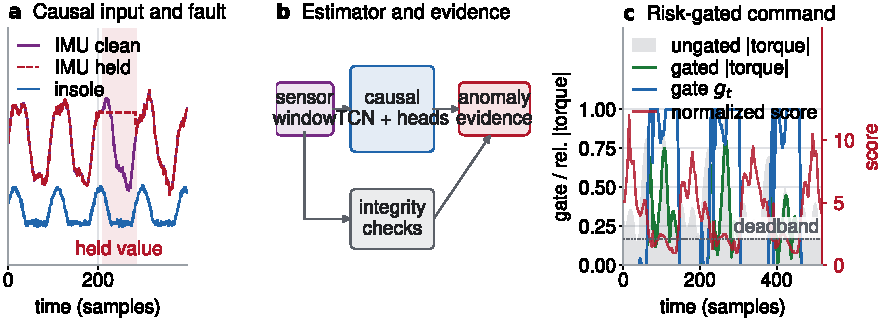
\includegraphics[width=\textwidth]{figures/fig_method_overview.pdf}
\caption{Method overview. (a) Causal wearable input streams and locally plausible faults; traces are illustrative, with a held-value interval shaded. (b) A shared causal TCN predicts hip--knee moments and learned reliability evidence, while integrity checks target specific fault mechanisms; calibration, detector selection, and gate tuning use validation data only. (c) Measured per-timestep export from the seed-7 model on a held-in test window with \texttt{encoder\_dropout} injected: the gate attenuates the baseline command whenever fused risk exceeds the deadband and returns to one as risk falls back.}
\label{fig:overview}
\end{figure*}

\subsection{Reliability-Aware Causal TCN}

Training-participant channel means $\mathbf{c}$ and standard deviations $\mathbf{v}\in\mathbb{R}^{C}$ normalize each observation as
\begin{equation}
    \mathbf{z}_t=(\mathbf{x}_t-\mathbf{c})\oslash
    \max(\mathbf{v},10^{-6}),
\end{equation}
where $\oslash$ is elementwise division.
Following \citet{molinaro2024task} and \citet{bai2018tcn}, the shared encoder has $L=5$ residual blocks, each with two causal convolutions of kernel size $k=5$ and dilation $2^{\ell-1}$, weight normalization, ReLU, and spatial dropout.
The receptive field is
\begin{equation}
    H=1+2(k-1)\sum_{\ell=1}^{L}2^{\ell-1}=249
\end{equation}
samples; the first $H-1$ window outputs are excluded from training and evaluation.

Five $1\!\times\!1$ heads produce the moment mean $\boldsymbol{\mu}_t$, log variance $\mathbf{s}_t$, binary fault logit $a_t$, clean-input reconstruction $\widehat{\mathbf{z}}_t$, and $h$-step forecast $\overline{\mathbf{z}}_{t+h\mid t}$.
We clamp $\mathbf{s}_t$ to $[-8,5]$ and define the diagonal predictive distribution
\begin{equation}
    p(\mathbf{y}_t\mid\widetilde{\mathbf{x}}_{1:t})
    = \mathcal{N}\!\left(\boldsymbol{\mu}_t,
      \operatorname{diag}(\exp\mathbf{s}_t)\right).
\end{equation}

\subsection{Fault-Augmented Multi-Task Learning}

For each training window, we sample clean data or one of six faults: missing insole, encoder dropout, IMU bias, packet loss, stuck IMU, or sensor delay.
The operator $\widetilde{\mathbf{x}}=\mathcal{A}_f(\mathbf{x};\boldsymbol{\xi})$ zeros missing modalities, applies a variance-scaled bias ramp, holds the previous value after packet loss, or shifts modalities by different delays to create asynchrony.
Every generator has a fixed severity and target group: the insole and encoder groups are zeroed outright; the shank IMU takes a bias ramp of $0.25$ channel standard deviations and the thigh IMU an axis-scale error of $0.35$; packet loss holds each sample independently with probability $0.15$ across all groups; the foot IMU freezes for the stuck-IMU case; and sensor delay shifts every group by $10$ samples ($50$~ms) scaled per group by $1.0$, $1.6$, $0.6$, $2.0$, and $1.2$ for foot, shank, thigh, insole, and encoder, so the modalities become mutually asynchronous rather than uniformly late.
Each fault occupies its whole window, so the fault label $b_f$ below is window-constant.
The three held-out generators reuse the same rates through different mechanisms: burst loss drops runs of $\max(2,\operatorname{round}(2+24p))$ samples at rate $p$, partial loss draws an independent mask per channel, and delay jitter redraws the shift per window in $[0.5,1.5]$ times nominal.

Let $m_{jt}$ indicate whether a moment label is valid, and let $b_f=\mathbb{I}[f\neq\mathrm{clean}]$.
The masked heteroscedastic loss is
\begin{equation}
\begin{aligned}
\mathcal{L}_{\mathrm{mom}}
&=\frac{1}{2\sum_{j,t}m_{jt}}\sum_{j,t}m_{jt}\,\ell_{jt},\\
\ell_{jt}&=s_{jt}+(y_{jt}-\mu_{jt})^2\exp(-s_{jt}).
\end{aligned}
\end{equation}
The moment head receives $\widetilde{\mathbf{x}}$ with the clean target $\mathbf{y}$, encouraging robustness when a fault leaves enough information.
The fault head is optimized using timestepwise binary cross-entropy:
\begin{equation}
\begin{aligned}
\mathcal{L}_{\mathrm{fault}}=-\frac{1}{|\Omega|}\sum_{t\in\Omega}
\big[&b_f\log\sigma(a_t)\\
&+(1-b_f)\log(1-\sigma(a_t))\big],
\end{aligned}
\end{equation}
where $\Omega$ contains the timesteps with at least one valid joint label.

The auxiliary heads recover the uncorrupted normalized sequence instead of reproducing the corrupted input:
\begin{align}
\mathcal{L}_{\mathrm{rec}} & = \operatorname{MSE}_{\Omega}
\left(\widehat{\mathbf{z}}_t(\widetilde{\mathbf{x}}),\mathbf{z}_t(\mathbf{x})\right),\\
\mathcal{L}_{\mathrm{pred}} & = \operatorname{MSE}_{\Omega}
\left(\overline{\mathbf{z}}_{t+h\mid t}(\widetilde{\mathbf{x}}_{1:t}),\mathbf{z}_{t+h}(\mathbf{x})\right).
\end{align}
The complete objective is
\begin{equation}
    \mathcal{L}=\mathcal{L}_{\mathrm{mom}}+
    \lambda_f\mathcal{L}_{\mathrm{fault}}+
    \lambda_r\mathcal{L}_{\mathrm{rec}}+
    \lambda_p\mathcal{L}_{\mathrm{pred}},
\end{equation}
with $(\lambda_f,\lambda_r,\lambda_p)=(0.2,0.1,0.1)$.
Reconstruction updates the shared encoder, whereas forecasting stops gradients at $\mathbf{h}_t$ so that it acts as a temporal probe.

\subsection{Complementary Integrity Signals}

Different faults affect different signal properties, so the monitor considers eight candidate signals.
The learned signals are fault probability $q_t^{\mathrm{fault}}=\sigma(a_t)$, mean aleatoric scale $q_t^{\mathrm{ale}}=\frac{1}{2}\sum_j\exp(s_{jt}/2)$, reconstruction and forecast residuals, and optional epistemic scale.
For a modality group $G$, the residual scores are
\begin{align}
q_t^{\mathrm{rec}} &= \max_G\frac{1}{|G|}\sum_{c\in G}
(\widehat z_{ct}-\widetilde z_{ct})^2,\\
q_{t+h}^{\mathrm{pred}} &= \max_G\frac{1}{|G|}\sum_{c\in G}
(\overline z_{c,t+h\mid t}-\widetilde z_{c,t+h})^2.
\end{align}
A forecast made at $t$ is scored only when its target arrives at $t+h$, so risk at $u$ compares $\overline{\mathbf{z}}_{u\mid u-h}$ with $\widetilde{\mathbf{z}}_u$ and the channel is zero for the first $h$ samples, preserving command-time causality.
Epistemic scale is the joint-averaged standard deviation across stochastic-dropout passes or ensemble members.

Three causal statistics cover signatures that learned heads may miss. Staleness is the moving fraction of nearly unchanged channels. Coherence is one minus the mean absolute rolling correlation between differenced, corresponding IMU axes. Drift is the largest modality-averaged channel slope.
Coherence and drift are offline diagnostic channels and are not used by the command-time gate.

\subsection{Validation-Calibrated Fault Detection}

For validation window $i$, each channel is averaged over its valid timesteps $\Omega_i$ to obtain $Q_{ik}=|\Omega_i|^{-1}\sum_{t\in\Omega_i}q_{it}^{k}$.
We define the detector reference using clean validation windows as
\begin{equation}
    \rho_k^{\mathrm{det}}=\operatorname{Quantile}_{0.9}
    \left(\{Q_{ik}:i\in\mathcal{V}_{\mathrm{clean}}\}\right)
\end{equation}
and fuse a subset $S$ according to
\begin{equation}
    R_i^{\mathrm{det}}(S) = \max_{k\in S}
    Q_{ik}/\max(\rho_k^{\mathrm{det}},10^{-6}).
\end{equation}
Using validation faults only, we enumerate subsets of at most three channels and, given their validation-fault AUROCs $A_f(S)$, maximize
\begin{equation}
    J_{\mathrm{det}}(S)=\operatorname{mean}_f A_f(S)
    +0.25\min_f A_f(S)-0.002(|S|-1),
\end{equation}
where the second term rewards the hardest fault and the last favors smaller subsets.
Both $S$ and $\rho_k^{\mathrm{det}}$ are frozen before test evaluation, and burst packet loss, independent partial-channel loss, and randomized delay jitter are excluded from training and detector selection alike.

\subsection{Utility-Aware Assistance Gate}

The command-time risk uses the causal timestep-level channels
$\mathcal{K}_{\mathrm{gate}}=\{\mathrm{fault},\mathrm{ale},\mathrm{rec},\mathrm{pred},\mathrm{epi},\mathrm{stale}\}$ that are available in a given configuration:
\begin{equation}
    r_t=\max_{k\in\mathcal{K}_{\mathrm{gate}}}
    q_t^k/\max(\rho_k^{\mathrm{gate}},10^{-6}).
\end{equation}
We share the detector scale, $\rho_k^{\mathrm{gate}}:=\rho_k^{\mathrm{det}}$, to keep window- and timestep-level scores comparable; it is not a timestep-score quantile.
Clean held-out-task validation trials and designated validation faults instead calibrate the deadband $d$ and softness $\gamma$.

The risk is converted into a continuous gain:
\begin{equation}
g_t = \operatorname{clip}_{[0,1]}\!\left(
1-\frac{r_t-(1+d)}{\gamma}\right),
\end{equation}
so $g_t=1$ within the nominal region $r_t\leq1+d$ and decreases linearly beyond it.
Starting from $d_0=0.1$, we set
\begin{equation}
    d=\min\!\left(d_{\max},\max\left[d_0,
    \operatorname{Quantile}_{0.9}(r^{\mathrm{val\text{-}OOD}})-1\right]\right),
\end{equation}
with $d_{\max}=2$, using clean held-out-task trials from validation participants.
We then search $\gamma\in\{0.25,0.5,1,2,4,8\}$.
Feasible values retain at least 95\% of clean aligned torque, meet the clean wrong-direction tolerance, and do not increase wrong-direction torque under validation faults.
Writing $\kappa_{\mathrm{clean}}$ for gated-over-ungated clean retention and, averaged over validation faults, $\bar\delta$ for the relative wrong-direction reduction $\min(1,\max(0,1-w^{\mathrm{gated}}/w^{\mathrm{ungated}}))$ and $\bar\kappa$ for fault retention, feasible pairs are ranked by
\begin{equation}
    J_{\mathrm{gate}} = \kappa_{\mathrm{clean}} + 2\bar\delta + 0.25\,\bar\kappa,
\end{equation}
so safety dominates but is not bought by closing the gate outright; infeasible pairs are rejected.

The baseline transformation $\mathcal{C}$ scales the estimated hip and knee moments by $0.20$ and $0.15$, applies the configured joint delays and a 6-Hz low-pass filter, and clips torque to $0.45$ Nm/kg; the gated command is $\boldsymbol{\tau}^{\mathrm{cmd}}_t=g_t\mathcal{C}(\boldsymbol{\mu}_{1:t})$.
This policy attenuates commands derived from unreliable estimates but does not replace independent actuator saturation or hardware limits.

\section{Experimental Protocol}
\subsection{Data, Splits, and Comparisons}

We use the released exoskeleton sensor and biological-moment data underlying the task-agnostic controller \citep{molinaro2024task,scherpereel2023dataset}, resampled to a uniform $200$~Hz, so one sample is $5$~ms and the forecast horizon $h=1$ is one control step.
Inputs comprise $25$ unilateral channels in five modality groups $G$: foot, shank, and thigh IMU ($6$ channels each, three gyroscope and three accelerometer axes), insole ($3$), and hip--knee encoders ($4$); the action profiles of the input ablation add a sixth group. Targets are right hip and knee moments in Nm/kg.
Of the $15$ participants, $11$ train, $2$ validate, and $2$ test, and jumping, cutting, weight lifting, and lunges are reserved as task OOD; no test participant informs preprocessing, calibration, detector selection, or gate tuning.
The leave-one-subject-out analysis rotates over all $15$ participants, giving $15$ folds, each with the preceding participant as validation.
The primary baseline is a deterministic, non-augmented TCN on the same split; the released Nature checkpoint is contextual because its split differs.
Ablations add fault augmentation, probabilistic regression, reconstruction, and forecasting in order, with additional dropout, ensemble, action-input, severity, and leave-one-subject-out analyses.

\subsection{Metrics and Implementation}

We report RMSE, MAE, $R^2$, Gaussian NLL, uncertainty--error correlation, interval coverage and calibration error, and per-channel and fused fault AUROC.
The control-replay metrics are defined against the ideal command $\boldsymbol{\tau}^{\star}=\mathcal{C}(\mathbf{y})$ obtained by passing the \emph{true} moment through the same transformation $\mathcal{C}$.
A joint-timestep pair $n$ is \emph{active} when its label is valid and $|\tau^{\star}_n|>0.02$ Nm/kg; the resulting set $\mathcal{A}$ depends only on the true moment, so it is identical for the gated and ungated commands and cannot be shrunk by attenuation.
Writing $u_n=\tau^{\mathrm{cmd}}_n$, the wrong-direction ratio $w$ and retained aligned torque $\kappa$ are
\begin{align}
w &= \tfrac{1}{|\mathcal{A}|}\textstyle\sum_{n\in\mathcal{A}}
     \mathbb{I}[u_n\tau^{\star}_n<0],\\
\kappa &= \frac{\sum_{n\in\mathcal{A}}\max(0,\,u_n\operatorname{sgn}\tau^{\star}_n)}
       {\sum_{n\in\mathcal{A}}|\tau^{\star}_n|},
\end{align}
and we also report the peak $|u_n|$ over wrong-direction steps and the mean absolute command jerk.
Since $u_n=g_t\mathcal{C}(\boldsymbol{\mu})_n$ with $g_t\geq0$, scaling never flips a sign: every reduction in $w$ comes from steps where $g_t$ reaches exactly zero, and $\kappa$ is the price paid for them, so neither quantity can be improved by simply lowering the gate and both must be reported.
A first-order actuator proxy also estimates net-moment RMS and work-related quantities; these are relative offline comparisons, not measured metabolic outcomes.
The model has five 80-channel TCN blocks, kernel size 5, dropout 0.15, and 768-sample windows at stride 384, with the first 248 outputs masked.
We train for 20 epochs with Adam ($10^{-3}$) using seeds 7, 13, and 23 and report mean, standard deviation, and paired seed-level differences.
Three seeds quantify only training stochasticity, so the interval estimate for the main safety claim instead comes from the fifteen leave-one-subject-out folds, as a percentile bootstrap $95\%$ confidence interval over folds ($10{,}000$ resamples, fixed seed) on the per-subject wrong-direction reduction.
We report no per-scenario significance tests: over ten scenarios, two splits, and several metrics, an uncorrected family would be uninterpretable and a corrected one underpowered at three seeds, so per-scenario entries are descriptive and the confirmatory claim rests on that single pre-specified between-subject interval.

\section{Results}

Unless stated otherwise, entries are means and standard deviations over seeds 7, 13, and 23, and all detector and gate choices remain fixed from validation data.

\subsection{Moment Accuracy and Calibration}

Table~\ref{tab:accuracy} compares the proposed model with the split-matched deterministic TCN on uncorrupted trials.
On ID tasks, reliability training changes RMSE from $0.1616\pm0.0008$ to $0.1726\pm0.0017$ Nm/kg (paired difference $+0.0110\pm0.0024$); the corresponding OOD values are $0.2319\pm0.0050$ and $0.2531\pm0.0023$ Nm/kg ($+0.0213\pm0.0045$).
Coverage ECEs of the probabilistic model are $0.033\pm0.017$ and $0.028\pm0.010$.
Reliability training therefore trades some clean accuracy for fault robustness rather than improving both criteria; the released Nature checkpoint appears only as contextual reference because its split is not matched to ours.

\begin{table}[t]
\centering
\scriptsize
\setlength{\tabcolsep}{1.8pt}
\begin{tabular}{lcccc}
\toprule
Method & RMSE & $R^2$ & NLL & ECE\\
\midrule
\multicolumn{5}{l}{ID tasks}\\
Det. TCN & $0.162\pm0.001$ & $0.798\pm0.002$ & -- & --\\
Proposed & $0.173\pm0.002$ & $0.770\pm0.005$ & $-1.453\pm0.034$ & $0.033\pm0.017$\\
\addlinespace[2pt]
\multicolumn{5}{l}{Held-out tasks (OOD)}\\
Det. TCN & $0.232\pm0.005$ & $0.751\pm0.011$ & -- & --\\
Proposed & $0.253\pm0.002$ & $0.704\pm0.005$ & $-1.063\pm0.022$ & $0.028\pm0.010$\\
\bottomrule
\end{tabular}
\caption{Clean moment estimation and calibration on unseen participants, reported as mean $\pm$ standard deviation over three seeds. RMSE is in Nm/kg. Lower is better for RMSE, NLL, and ECE; higher is better for $R^2$. NLL and ECE are not defined for the deterministic TCN.}
\label{tab:accuracy}
\end{table}

\subsection{Fault Detection under Task Shift}

Figure~\ref{fig:detection-taxonomy} reports representative per-fault AUROC values for the frozen fused detector and its candidate channels.
Across the six reported training-time fault types, the fused detector reaches macro-AUROC $0.849\pm0.005$ on ID tasks and $0.773\pm0.002$ on held-out tasks.
For the unseen burst, partial-loss, and delay-jitter generators, the corresponding macro-AUROCs are $0.842\pm0.010$ and $0.778\pm0.004$.
The strongest individual signal is coherence, which reaches $1.000$ AUROC for both partial channel loss and a stuck IMU on ID and OOD tasks, whereas IMU bias remains the most difficult fused case at $0.502$ and $0.504$ AUROC.
Reporting each fault separately prevents aggregate AUROC from hiding systematic detector failures.

\begin{figure*}[t]
\centering
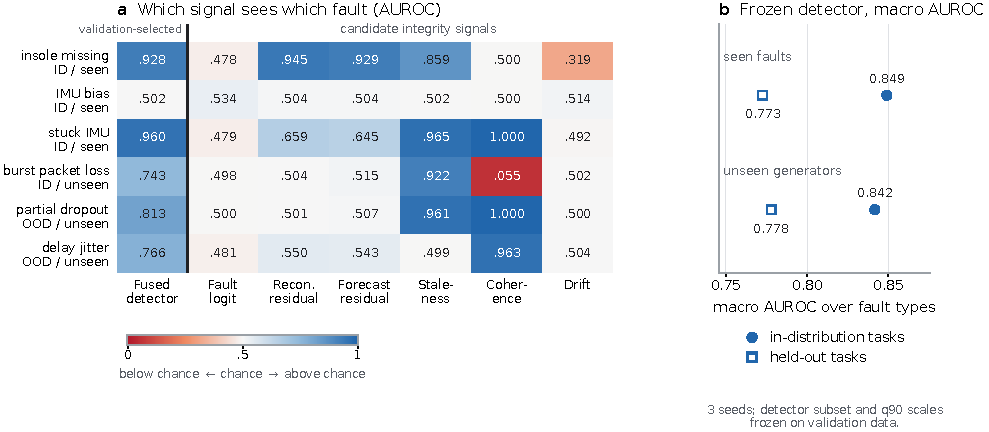
\includegraphics[width=\textwidth]{figures/fig_detection_taxonomy.pdf}
\caption{Fault-mechanism detectability across complementary signals. (a) Clean-versus-fault AUROC per candidate signal and for the frozen fused detector, separated at the left because its subset and scales are fixed on validation data. Color diverges about chance ($0.500$ neutral); row labels give the fault and whether its generator was seen in training. (b) Macro AUROC of the frozen detector over fault types: circles for in-distribution, squares for held-out tasks (mean over three seeds).}
\label{fig:detection-taxonomy}
\end{figure*}

\subsection{Safety--Utility Trade-off}

% 浮动体声明放在首次引用它的段落之前。LaTeX 不会把浮动体排到声明点之前，
% 声明得晚就只剩下末尾几个页顶可用：figures 4/5 因此被推到两个纯浮动页上，
% 正文到第 7 页就结束了，整篇却占 10 页。
\begin{figure*}[t]
\centering
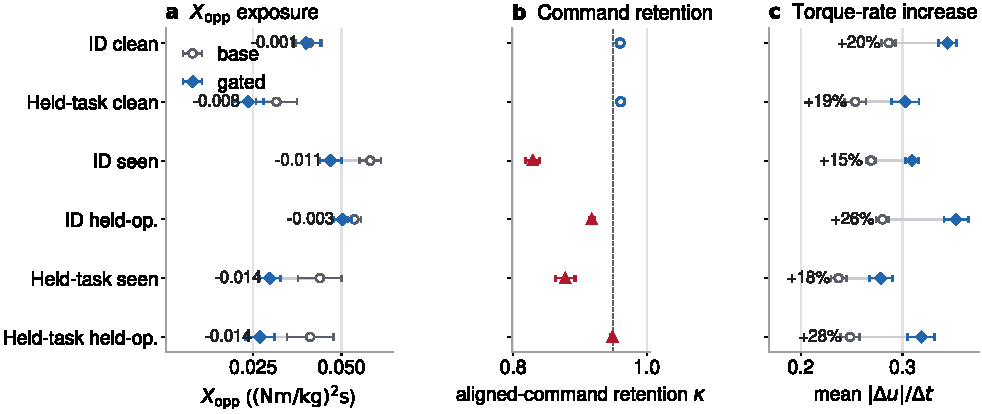
\includegraphics[width=\textwidth]{figures/fig_safety_utility.pdf}
\caption{Control consequences of the frozen gate. (a) Paired markers compare the ungated and gated wrong-direction ratio per scenario; direct labels give the paired change in percentage points. (b) The safety--utility plane places wrong-direction reduction against retained aligned torque, with open circles for clean trials and filled triangles for faulty ones; the dashed line marks the $95\%$ clean-retention constraint used during validation. (c) Mean gate value over active steps for the same scenarios.}
\label{fig:safety-utility}
\end{figure*}

Figure~\ref{fig:safety-utility} compares the estimator before and after the frozen gate; changes in $w$ are differences between fractions of active timesteps, so $-0.0074$ is $-0.74$ percentage points.
On clean ID and OOD trials the gate retains $0.960$ and $0.961$ of aligned assistance at wrong-direction changes of $-0.0005$ and $-0.0074$.
Across training-time fault types the ratio changes by $-0.0052$ on ID and $-0.0109$ on OOD tasks; for unseen generators, $-0.0017$ and $-0.0103$.
Mean gate values stay between $0.904$ and $0.978$, so the reduction comes from selective attenuation rather than a near-closed gate, and the paired retention figures bound its cost.
Actuator-replay outcomes are reported only as offline proxies.

\subsection{Ablations and Stress Tests}

\begin{figure*}[t]
\centering
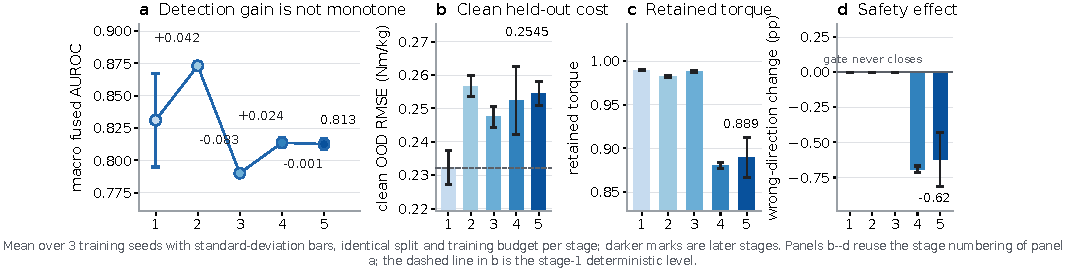
\includegraphics[width=\textwidth]{figures/fig_ablation_summary.pdf}
\caption{Ordered component attribution on a fixed data split and training budget. Stages are numbered 1--5 as fault augmentation, probabilistic regression, reconstruction, and forecasting are added in sequence, and panels (b)--(d) reuse that numbering. (a) Macro fault AUROC per stage, with signed annotations for each adjacent step. (b) Clean OOD RMSE; the dashed rule is the deterministic stage-1 level. (c) Retained aligned torque and (d) wrong-direction change in percentage points under each stage's own validation-selected gate, both macro-averaged over the fixed fault set. Stages 1--3 select a deadband their risk never exceeds, so their gate never closes and panel (d) is identically zero there: detection quality at those stages has no actuation consequence. Entries are means over three training seeds; bars give the cross-seed standard deviation.}
\label{fig:ablation-summary}
\end{figure*}

Figure~\ref{fig:ablation-summary} follows a fixed attribution sequence specified before the sweep, and reports each adjacent step as a seed-paired change over three seeds so stage effects can be compared against training variability.
Fault augmentation changes macro fault AUROC by $+0.042 \pm 0.036$ and clean OOD RMSE by $+0.025 \pm 0.008$ Nm/kg; that AUROC change is of the same order as the seed spread of the deterministic stage itself ($0.831 \pm 0.036$), so the first step remains diagnostic rather than a firm ranking.
Adding probabilistic prediction, reconstruction, and forecasting produces successive AUROC changes of $-0.083 \pm 0.003$, $+0.024 \pm 0.004$, and $-0.001 \pm 0.008$; the first two exceed seed noise by an order of magnitude, while the last is within it.
Detection quality alone would therefore rank stage 2 highest, but panel (d) shows that stages 1--3 carry no safety effect at all: each selects a deadband from its own validation risk that its test risk never exceeds, so $g_t\equiv1$ and the wrong-direction change is exactly $0$ in every evaluated scenario, with retained torque correspondingly near $0.99$.
Only once the reconstruction residual enters the risk does the gate close, at a wrong-direction change of $-0.69\pm0.02$ percentage points and retained torque $0.881 \pm 0.003$; forecasting keeps that effect at $-0.62\pm0.19$ points with retention $0.889 \pm 0.023$.
An ablation read on AUROC alone would thus promote a control-inert configuration, which is why the attribution is reported jointly with the actuation outcome.

% 单栏图允许排在栏底，多给一个候选位置。figure* 不能用 b（那需要 stfloats，
% AAAI 样式明确禁用），所以只有这一张能这样放。
\begin{figure}[tb]
\centering
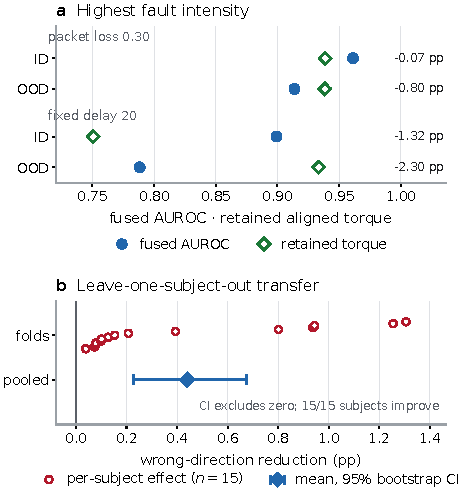
\includegraphics[width=\columnwidth]{figures/fig_stress_transfer.pdf}
\caption{Severity extremes and subject transfer. (a) At the highest packet-loss rate and the longest fixed delay, filled circles give fused AUROC and open diamonds the retained aligned-torque ratio on the same axis; labels give the wrong-direction change in percentage points. (b) Each open circle is one leave-one-subject-out fold; the diamond is the mean with its $95\%$ bootstrap interval over $15$ folds. The interval excludes zero and every fold improves, but fold magnitudes span roughly a factor of thirty.}
\label{fig:stress-transfer}
\end{figure}

Figure~\ref{fig:stress-transfer} tests the operating point more strictly than a single severity does.
At the largest packet-loss rate, fused AUROC is $0.961$ on ID and $0.914$ on OOD tasks, with retained ratios $0.939$ and $0.938$ and wrong-direction changes of $-0.0007$ and $-0.0080$; at the longest fixed delay, AUROC is $0.899$ and $0.788$, retention $0.751$ and $0.933$, and the changes $-0.0132$ and $-0.0230$.
Adding desired, measured, execution, or interaction torque to the $25$-channel human-only input moves ID macro AUROC only from $0.843$ to $0.842$--$0.847$ and held-out AUROC from $0.774$ to $0.771$--$0.784$, while clean OOD RMSE rises from $0.251$ to $0.259$--$0.278$ Nm/kg: no reliable gain, and not the ID-only pattern a device-specific shortcut would show, so the human-only set is retained.
A three-member deep ensemble raises the epistemic channel from $0.497$ to $0.553$ AUROC on seen ID faults but leaves the fused detector unchanged ($0.843$ versus $0.842$ on ID, $0.771$ on OOD) because the frozen fusion never selects it, tripling inference cost without moving the operating point.
Across the fifteen leave-one-subject-out folds, the per-subject wrong-direction reduction averages $0.44$ percentage points with a $95\%$ bootstrap interval of $[0.23,0.67]$ points over $10{,}000$ resamples; the interval excludes zero and all $15$ folds improve, with a between-subject standard deviation of $0.47$ points and a range of $0.04$ to $1.31$.
Mean clean retention across folds is $0.961$ and never falls below $0.880$, so the reduction is not obtained by withdrawing assistance; it is largest for encoder dropout and delay and smallest for packet loss and IMU bias, consistent in sign but varying several-fold in size.

\section{Discussion}
Reliability estimates matter only if they change the command rather than serving as confidence scores.
The validation-calibrated gate reduces wrong-direction assistance under non-clean conditions by about $0.007$ absolute while retaining $96.1\%$ of clean aligned torque: a modest improvement at one operating point, not a safety guarantee, but one obtained without turning assistance off.
Since AUROC does not measure control consequences, both wrong-direction torque and retained assistance are needed to expose that trade-off, and the ablation shows the two can move independently.

Fault mechanisms violate different signal properties: reconstruction is most informative for missing insole, staleness for packet loss, and coherence for partial channel loss and delay.
Fusion covers more cases, but IMU bias remains near chance, suggesting slow bias is close to indistinguishable from valid motion with these sensors.
Some auxiliary heads also reduce the aggregate well outside seed noise, and clean RMSE is worse than the split-matched deterministic TCN, so predictive uncertainty and auxiliary training are not universal solutions; bias-sensitive checks and loss balancing remain open.

The method complements the two baseline directions rather than replacing them: task-agnostic estimation expands behavioral coverage \citep{molinaro2024task}, domain adaptation reduces training-data demands \citep{scherpereel2025domain}, and this gate addresses corrupted observations after deployment.
A domain-adapted estimator could reuse the monitor, but its calibration would have to be repeated in the target sensor domain, and applications with different actuator authority should pick a new point on the validation trade-off rather than reuse the reported threshold.


\section{Limitations}
The reported reduction is not attributable to fault detection alone.
On clean held-out-task trials, where no fault is present, gating still lowers wrong-direction torque by $0.74$ percentage points, which is the same order as the $1.09$ and $1.03$ points obtained on faulty held-out trials.
The risk channels respond to prediction error in general, so an unknown part of the aggregate effect suppresses ordinary task-shift error rather than sensor failure; separating the two would require a fault-free OOD control condition that our current protocol does not isolate.
The evaluated faults are synthetic and cannot represent the complete hardware failure distribution.
We did not run the reliability gate online on a physical exoskeleton or conduct a closed-loop human-subject experiment.
The actuator replay assumes fixed recorded kinematics and supports relative comparisons, not claims about interaction safety, human adaptation, or metabolic benefit.
Moment labels and sensing originate from one exoskeleton platform, and the current implementation does not jointly train the domain-adaptation model from \citet{scherpereel2025domain}.
A gate can reduce exposure to a detected failure but cannot guarantee safety under an undetectable or adversarial fault. Independent low-level torque and hardware limits remain necessary.

\section{Ethical Statement}

Reliability-aware assistance may reduce risk from silent sensing failures, but overconfident claims could encourage premature deployment around human users.
We distinguish offline replay from human-subject evidence, report negative and weak detector results, and do not present the learned gate as a formal safety guarantee.
Released participant data must be handled under the terms and consent conditions of the source dataset.

\section{Conclusion}
We presented a reliability layer that combines learned outputs with causal integrity signals and uses validation-calibrated risk to attenuate moment-based assistance.
The evaluation separates participant, task, and sensor-fault shifts and reports both the reduction in harmful torque and the assistance lost in exchange.
Future work will target the weak detection of slow bias and validate the complete monitor and fallback policy in real-time exoskeleton experiments with human participants, which is required before the method is used outside controlled sensor conditions.

% Anonymous submission: acknowledgments intentionally omitted.

\bibliography{references}

\end{document}
